% ============================================================
% Bachelor Thesis - Technische Hochschule Ingolstadt / CARISSMA
% Title: Identification and Interpretation of BMS Signals Through
%        CAN Bus Reverse Engineering on the VW ID. Buzz
% Author: Muhamad Alif Izzuwan Bin Ibrahim
% Layout closely follows the THI/Carissma reference format.
% ============================================================

\documentclass[11pt,a4paper,oneside,parskip=half]{scrreprt}

% ---------- Encoding / Language ----------
\usepackage[utf8]{inputenc}
\usepackage[T1]{fontenc}
\usepackage[english]{babel}
% ---------- Garamond body font (11 pt, set on the documentclass line) ----------
\usepackage{ebgaramond}              % EB Garamond for the body text
\usepackage[cmintegrals,cmbraces]{newtxmath} % math that pairs with Garamond
\usepackage{microtype}

% ---------- Page geometry (matches reference) ----------
\usepackage[
  a4paper,
  top=2.5cm,
  bottom=2.5cm,
  left=3.0cm,
  right=2.5cm,
  headheight=15pt,
  headsep=0.6cm,
  footskip=1.2cm
]{geometry}

\usepackage{setspace}
\setstretch{1.25}   % 1.25 line spacing

% ---------- Graphics, figures, tables ----------
\usepackage{graphicx}
\graphicspath{{figures/}{fig/}}
\usepackage{float}
\usepackage{caption}
\usepackage{subcaption}
\captionsetup{font=small,labelfont=bf,labelsep=colon,justification=raggedright,singlelinecheck=false}

\usepackage{booktabs}
\usepackage{tabularx}
\usepackage{longtable}
\usepackage{multirow}
\usepackage{array}
\newcolumntype{C}[1]{>{\centering\arraybackslash}p{#1}}
\newcolumntype{L}[1]{>{\raggedright\arraybackslash}p{#1}}

% ---------- Math & units ----------
\let\Bbbk\relax           % avoid clash between newtxmath and amssymb
\usepackage{amsmath,amssymb}

% ---------- Colour & TikZ ----------
\usepackage[dvipsnames,table]{xcolor}
\usepackage{tikz}
\usetikzlibrary{shapes.geometric,arrows.meta,positioning,calc,fit,matrix,decorations.pathreplacing}

% ---------- Code listings ----------
\usepackage{listings}
\lstset{
  basicstyle=\ttfamily\footnotesize,
  breaklines=true,
  frame=single,
  numbers=left,
  numberstyle=\tiny\color{gray},
  keywordstyle=\bfseries,
  commentstyle=\itshape\color{gray!70!black},
  backgroundcolor=\color{gray!5},
  tabsize=2,
  showstringspaces=false,
  captionpos=b,
  xleftmargin=1em,
}

% ---------- Headers and footers (reference style) ----------
\usepackage{fancyhdr}

% Define chapter header mark: "CHAPTER 1. INTRODUCTION"
\renewcommand{\chaptermark}[1]{\markboth{CHAPTER \thechapter.\ \MakeUppercase{#1}}{}}
\renewcommand{\sectionmark}[1]{}

\pagestyle{fancy}
\fancyhf{}
\fancyhead[R]{\small\textsc{\leftmark}}
\fancyfoot[L]{\small Muhamad Alif I.~B.~Ibrahim}
\fancyfoot[C]{\small\thepage}
\fancyfoot[R]{\small THI / Carissma}
\renewcommand{\headrulewidth}{0.5pt}
\renewcommand{\footrulewidth}{0pt}

\fancypagestyle{plain}{%
  \fancyhf{}
  \fancyfoot[L]{\small Muhamad Alif I.~B.~Ibrahim}
  \fancyfoot[C]{\small\thepage}
  \fancyfoot[R]{\small THI / Carissma}
  \renewcommand{\headrulewidth}{0pt}
}

% ---------- Hyperref (kept plain, black links for print) ----------
\usepackage[hidelinks,
  pdftitle={Identification and Interpretation of BMS Signals Through CAN Bus Reverse Engineering on the VW ID. Buzz},
  pdfauthor={Muhamad Alif Izzuwan Bin Ibrahim},
  pdfsubject={Bachelor Thesis - Technische Hochschule Ingolstadt},
  pdfkeywords={CAN, UDS, OBD-II, BMS, Volkswagen, ID. Buzz, reverse engineering}
]{hyperref}

% ---------- KOMA typography: unbold chapter numbers look plain ----------
\addtokomafont{disposition}{\rmfamily}
\setkomafont{chapter}{\normalfont\bfseries\Large}
\setkomafont{section}{\normalfont\bfseries\large}
\setkomafont{subsection}{\normalfont\bfseries\normalsize}
\RedeclareSectionCommand[beforeskip=-0.5\baselineskip,afterskip=1.2\baselineskip]{chapter}

% ---------- Helper macros ----------
\newcommand{\canid}[1]{\texttt{0x#1}}
\newcommand{\udssid}[1]{\texttt{0x#1}}
\providecommand{\hex}{}\renewcommand{\hex}[1]{\texttt{0x#1}}
\newcommand{\byte}[1]{B[#1]}

% ============================================================
\begin{document}
% ============================================================

% ------------------------------------------------------------
% TITLE PAGE (matches reference layout)
% ------------------------------------------------------------
\pagenumbering{roman}
\setcounter{page}{1}
\thispagestyle{empty}

\begin{titlepage}
\thispagestyle{empty}
\begin{center}

% THI logo only, centred

\includegraphics[width=0.45\textwidth]{Technische_Hochschule_Ingolstadt_logo.svg.pdf}

\vspace{1.8cm}

{\large\textbf{Bachelorarbeit}}\\[0.9cm]

% Title
{\LARGE\bfseries Identification and Interpretation of BMS Signals}\\[0.4em]
{\Large\bfseries Through CAN Bus Reverse Engineering}\\[0.2em]
{\Large\bfseries on the Volkswagen ID.~Buzz}\\[1.4cm]

{\normalsize vorgelegt von}\\[0.6em]
{\Large\bfseries Muhamad Alif Izzuwan Bin Ibrahim}\\[1.4cm]

% Student details block, left-aligned
\begin{flushleft}
\hspace{1.2cm}
\begin{tabular}{@{}p{4.5cm}l@{}}
\textbf{Matrikelnummer:} & 00124399 \\[2pt]
\textbf{Studiengang:}    & Elektrotechnik und Elektromobilit\"at (B.~Eng.) \\[2pt]
\textbf{Fakult\"at:}     & Elektrotechnik und Informatik \\
\end{tabular}
\end{flushleft}

\vspace{1.0cm}

\begin{flushleft}
\hspace{1.2cm}
\begin{tabular}{@{}p{4.5cm}l@{}}
\textbf{Erstpr\"ufer:}  & Prof.\ Dr.\ rer.\ nat.\ Hans-Georg Schweiger \\[2pt]
\textbf{Zweitpr\"ufer:} & Prof.\ Dr.\ Werner Huber \\[2pt]
\textbf{Betreuer:}      & Markus Gregor \\
\end{tabular}
\end{flushleft}

\vspace{1.5cm}

{\normalsize Ausgabedatum: 10.03.2026}\\[2pt]
{\normalsize Abgabedatum: 15.07.2026}

\end{center}
\end{titlepage}

% ------------------------------------------------------------
% DECLARATION
% ------------------------------------------------------------
\chapter*{Declaration in accordance with \S18 (4) No.~7 APO THI}
\thispagestyle{plain}
\addcontentsline{toc}{chapter}{Declaration}

\noindent I hereby declare that I have written this thesis independently, that it has not previously been submitted for examination purposes elsewhere, that I have used no sources or aids other than those indicated, and that I have marked verbatim and paraphrased quotations as such.

\vspace{2.5cm}

\noindent
\begin{tabular}{@{}p{7cm}p{7cm}@{}}
\hrulefill & \hrulefill \\[-2pt]
\textbf{Place, Date} \hfill Ingolstadt, 15.07.2026 & \textbf{Signature} \\
\end{tabular}

% ------------------------------------------------------------
% ACKNOWLEDGEMENTS
% ------------------------------------------------------------
\chapter*{Acknowledgements}
\addcontentsline{toc}{chapter}{Acknowledgements}
\thispagestyle{plain}

The present work was carried out as part of my Bachelor studies in Electrical Engineering and Electric Mobility at Technische Hochschule Ingolstadt.

First and foremost, I would like to thank everyone who supported me during the preparation of this thesis. My sincere thanks go to Prof.\ Dr.\ Hans-Georg Schweiger for his weekly supervision and the regular consultation hours that provided invaluable guidance. I also thank Prof.\ Dr.\ Werner Huber for agreeing to act as second examiner and for the constructive feedback he provided on the scope of the work.

I am especially grateful to my supervisor Markus Gregor, who accompanied this work intensively and whose deep knowledge of the CARISSMA research environment shaped the experimental setup around the Volkswagen ID.~Buzz.

Finally, I would like to thank my parents, who believed in me throughout my studies and supported me both financially and morally during the long weeks of data collection and writing.

% ------------------------------------------------------------
% CONTENTS / LOF / LOT
% ------------------------------------------------------------
\tableofcontents
\addcontentsline{toc}{chapter}{Contents}

\listoffigures
\addcontentsline{toc}{chapter}{List of Figures}

\listoftables
\addcontentsline{toc}{chapter}{List of Tables}

\clearpage
\pagenumbering{arabic}
\setcounter{page}{1}

% ============================================================
\chapter{Introduction}
% ============================================================
This chapter gives an overview of the topic, the motivation, the problem statement and the structure of the thesis.

\section{Motivation}
In recent years, electric mobility has undergone an enormous change. Almost every established automotive manufacturer has announced a portfolio of battery-electric vehicles (BEVs), and governmental policy in the European Union has aligned fleet CO$_2$ targets with an electrified future~\cite{schaal2020meb}. Within these vehicles, the high-voltage traction battery is the single most expensive and safety-critical subsystem. Its operating state -- state of charge (SOC), state of health (SOH), pack voltage, pack current, cell temperatures and cell balancing status -- determines both the available driving range and the long-term reliability of the vehicle~\cite{xiong2018critical,park2021data}.

All of this information is exchanged inside the vehicle over the Controller Area Network (CAN)~\cite{iso11898}. However, the manufacturer-specific signal databases (DBC files) that describe how raw CAN frames map to physical quantities are proprietary and not publicly available. For independent researchers, safety labs such as CARISSMA and for fleet-operators who want to monitor their vehicles, this closed ecosystem is a significant obstacle: without signal definitions the raw CAN data is merely a stream of hexadecimal bytes without semantic meaning.

In principle, two approaches can recover this semantic layer. The first is \textit{passive reverse engineering}: tapping the raw battery CAN bus directly, recording a large amount of traffic and using statistical techniques to deduce what each byte represents. This approach, however, requires physical access to the internal battery-management bus on which the BMS broadcasts its raw frames. On the Volkswagen MEB platform that bus is \emph{not} exposed on the OBD-II connector: a central gateway ECU isolates the private vehicle buses, and for security reasons it does not forward the raw BMS broadcast frames to the externally accessible diagnostic bus. A passive byte-level reverse engineering of the BMS signals is therefore not feasible from the OBD-II port without invasively tapping the high-voltage battery wiring of the vehicle.

The second approach -- and the one pursued in this thesis -- is \textit{active diagnostic reverse engineering}: using the standardised Unified Diagnostic Services (UDS) protocol~\cite{iso14229} transported over ISO~15765-2 (ISO-TP)~\cite{iso15765} via the on-board diagnostic (OBD-II) connector~\cite{saej1962} to request specific Data Identifiers (DIDs) from the battery management ECU through the gateway. The gateway \emph{does} route addressed UDS diagnostic requests to the BMS, so the data becomes reachable. This is still a reverse-engineering task because the meaning, byte layout and scaling of these manufacturer-specific DIDs are undocumented and proprietary: each positive response is a stream of raw bytes whose physical interpretation must be recovered and then \textbf{validated by comparing the decoded value directly against the physical readings of the test vehicle} (dashboard SOC, measured pack voltage, ambient temperature, and so on).

The present work applies this approach to a Volkswagen ID.~Buzz built on the MEB platform. The ID.~Buzz represents Volkswagen's state-of-the-art modular electric architecture, which makes it a particularly interesting test object: its electric and electronic architecture is representative of the next decade of mass-market BEVs from the Volkswagen Group.

\section{Problem Statement}
The main goal of this thesis is to reverse engineer the high-voltage battery signals of a Volkswagen ID.~Buzz through its OBD-II diagnostic port. Because the raw BMS broadcast bus is isolated by the gateway, the work focuses on actively requesting battery Data Identifiers via the UDS protocol and recovering their physical meaning. The primary deliverable is the ability to request and decode the high-voltage battery parameters (in particular state of charge, pack voltage, cell voltages and cell-temperature statistics) and to confirm them against the physical state of the vehicle.

Within this overall objective the work addresses the following research questions:

\begin{enumerate}
  \item Which CAN bus is exposed on the OBD-II connector of the Volkswagen ID.~Buzz, and why are the raw BMS broadcast frames not directly observable on it?
  \item Which UDS services and Data Identifiers of the battery management ECU are reachable through the gateway from the OBD-II connector without a security-access unlock?
  \item How can the byte layout and scaling of these undocumented, manufacturer-specific DIDs be reverse engineered into physical battery parameters?
  \item How well do the decoded UDS values agree with the physical reference values of the test vehicle (dashboard SOC, measured pack voltage, ambient temperature), and where does the method reach its limits?
\end{enumerate}

\section{Structure of the Thesis}
This thesis is divided into six main chapters.

Chapter~1 gives an overview of the task and the structure of the thesis.

Chapter~2 presents the theoretical background by means of a literature review. It covers the CAN bus protocol, the OBD-II connector, the ISO-TP transport protocol, the UDS application layer, the Volkswagen MEB platform, traction-battery management systems in BEVs and the state of the art of CAN bus reverse engineering.

Chapter~3 describes the materials and methods used in this work. The test vehicle, the CANedge2 data logger, the OBD-II connection and the software tool chain based on \texttt{asammdf} and Python are documented, together with the UDS-based reverse-engineering methodology and the reasoning for using active diagnostics rather than passive bus tapping.

Chapter~4 presents the results: the UDS logging campaign, the response coverage, and the battery parameters decoded from the BMS and validated against the physical state of the vehicle.

Chapter~5 discusses the findings. The limitations of the approach and the comparison with related work are analysed, and practical applications are outlined.

Chapter~6 concludes the work and gives an outlook on future research directions.

% ============================================================
\chapter{Fundamentals and State of the Art}
% ============================================================
In this chapter the essential fundamentals for understanding this work are explained. The introduction serves to describe the Controller Area Network, the layered diagnostic protocol stack built on top of it (ISO-TP and UDS), the OBD-II interface, the Volkswagen MEB platform and the battery management subsystem of a modern BEV. The chapter closes with a short review of prior art in automotive CAN reverse engineering.

\section{Controller Area Network (CAN)}
The Controller Area Network was originally developed by Bosch in the 1980s and is today standardised in ISO 11898~\cite{iso11898}. It is a serial, differential, multi-master broadcast bus that has become the backbone of automotive embedded networking. Its key properties -- bit-wise, non-destructive arbitration, short message length, high reliability through CRC protection and low hardware cost -- make it extremely well suited to the distributed control problem of a modern vehicle~\cite{zimmermann2014bosch,reif2014automotive}.

\subsection{Physical and Link Layer}
On the physical layer, CAN uses a twisted differential pair (CAN-H and CAN-L) terminated with 120~$\Omega$ resistors at both ends. The bus is driven by each node through a transceiver that produces two complementary states: a \textit{dominant} state (logical 0) and a \textit{recessive} state (logical 1). A dominant bit always overrides a recessive one, which is the key mechanism for the arbitration scheme described below. For in-vehicle networks, bit rates of 500~kbit/s (high-speed CAN for powertrain) and 125~kbit/s (comfort CAN) are the most common values in the Volkswagen Group.

\subsection{Frame Structure}
Every CAN message is transmitted as a frame with the structure shown in Figure~\ref{fig:can_frame}. Apart from the start-of-frame bit, an 11-bit arbitration identifier (or 29-bit extended identifier), and control bits, the frame carries a payload of up to 8~bytes (Classical CAN; CAN-FD supports up to 64~bytes) protected by a 15-bit CRC.

\begin{figure}[H]
\centering
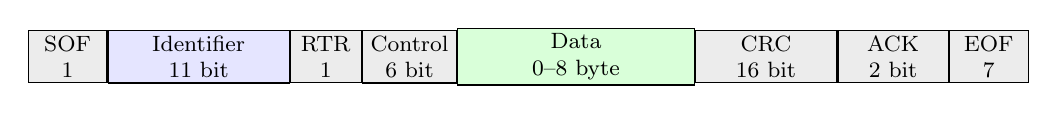
\begin{tikzpicture}[
  every node/.style={draw,minimum height=1.3em,font=\footnotesize,
    inner sep=2pt, align=center}]
\node[fill=gray!15,minimum width=1.0cm] (sof) {SOF\\1};
\node[right=0pt of sof,fill=blue!10,minimum width=2.3cm]  (id)  {Identifier\\11 bit};
\node[right=0pt of id,fill=gray!15,minimum width=0.9cm] (rtr) {RTR\\1};
\node[right=0pt of rtr,fill=gray!15,minimum width=1.2cm] (ctrl){Control\\6 bit};
\node[right=0pt of ctrl,fill=green!15,minimum width=3.0cm](data){Data\\0--8 byte};
\node[right=0pt of data,fill=gray!15,minimum width=1.8cm] (crc) {CRC\\16 bit};
\node[right=0pt of crc,fill=gray!15,minimum width=1.4cm] (ack) {ACK\\2 bit};
\node[right=0pt of ack,fill=gray!15,minimum width=1.0cm] (eof) {EOF\\7};
\end{tikzpicture}
\caption{Simplified layout of a classical CAN 2.0A data frame. The identifier field is used for bitwise arbitration; the data field carries the payload the application layer is interested in.}
\label{fig:can_frame}
\end{figure}

\subsection{Arbitration and Prioritisation}
CAN uses Carrier-Sense Multiple Access with Collision Resolution (CSMA/CR). When two or more nodes start transmitting simultaneously, each node reads back the bus level during its own transmission. Because a dominant bit (0) always wins over a recessive bit (1), the node with the numerically lower identifier automatically continues to transmit while the others switch to the listen state. This guarantees that the highest-priority message is never delayed by a collision. In an electric vehicle, safety-critical messages (such as the motor torque request or the battery current measurement) are therefore assigned low arbitration IDs, while convenience signals use higher IDs.

\subsection{Classical CAN vs.\ CAN-FD}
Two variants of the protocol are relevant. \textit{Classical CAN} (CAN~2.0, ISO~11898-1:2003) is limited to 8~payload bytes per frame and a single bit rate for the whole frame. \textit{CAN-FD} (CAN with Flexible Data-rate, standardised in ISO~11898-1:2015) extends this in two ways: the payload grows to up to 64~bytes, and the data phase of the frame may be transmitted at a higher bit rate than the arbitration phase, while the arbitration mechanism itself is unchanged.

The diagnostic CAN bus exposed on the OBD-II connector of the ID.~Buzz operates as a \textbf{Classical CAN bus at 500~kbit/s with 11-bit broadcast identifiers}; the diagnostic exchange with the battery ECU additionally uses 29-bit extended identifiers (Section~\ref{ssec:diag_addr}). It is \emph{not} CAN-FD. This is the decisive constraint behind the methodology of this thesis: because each frame carries at most 8~bytes, every UDS response longer than 7~payload bytes must be segmented by ISO-TP, and a logger that can only emit single CAN frames cannot read those multi-frame identifiers (Section~\ref{sec:uds_procedure}). The data logger used here (CANedge2) electrically supports both Classical CAN and CAN-FD, but is configured for Classical CAN at 500~kbit/s to match the vehicle, with the CAN-FD data bit rate left defined (2~Mbit/s) only so that the controller can initialise.

\section{Diagnostics: OBD-II, ISO-TP and UDS}
While the CAN bus is the low-level transport medium, automotive diagnostics rely on two additional layers built on top of CAN: a transport protocol that allows messages longer than 8~bytes to be fragmented and reassembled (ISO-TP), and an application layer that defines services, sub-functions and data identifiers (UDS). Both are accessed from outside the vehicle via a standardised connector: the OBD-II port.

It is useful to locate each of these protocols in the OSI reference model before going into detail, because the rest of the thesis repeatedly refers to ``which layer'' a given problem belongs to. The diagnostic stack used here maps onto the OSI layers as summarised in Table~\ref{tab:osi_stack}: CAN occupies the two lowest layers, ISO-TP provides the network/transport function that classical CAN itself lacks, and UDS is the application protocol that the battery management ECU actually speaks.

\begin{table}[H]
\caption{Mapping of the diagnostic protocol stack used in this thesis onto the OSI reference model.}
\label{tab:osi_stack}
\centering
\begin{tabular}{clp{6.6cm}}
\toprule
\textbf{OSI layer} & \textbf{Protocol} & \textbf{Role in this work} \\
\midrule
7 -- Application & UDS (ISO 14229)        & Services, sub-functions and Data Identifiers; \hex{22} \textit{ReadDataByIdentifier} returns the battery parameters. \\
6/5             & (not used)              & No presentation/session layer in CAN diagnostics. \\
4/3 -- Transport/Network & ISO-TP (ISO 15765-2) & Segments UDS messages longer than 7~bytes into First/Consecutive frames and reassembles them. \\
2 -- Data link  & CAN (ISO 11898-1)       & Frame format, arbitration, CRC, acknowledgement. \\
1 -- Physical   & CAN (ISO 11898-2)       & Differential CAN-H/CAN-L pair, 500~kbit/s, 120~$\Omega$ termination. \\
\bottomrule
\end{tabular}
\end{table}

\subsection{The OBD-II Connector (SAE J1962)}
All passenger cars sold in the European Union since 2004 (diesel: 2006) must expose a 16-pin diagnostic connector in the driver's footwell area, standardised by SAE J1962~\cite{saej1962}. Two pins carry the high-speed CAN bus used for emissions diagnostics (pin~6 = CAN-H, pin~14 = CAN-L). On many manufacturers' vehicles, additional pins are used by a \textit{gateway ECU} that multiplexes private manufacturer buses onto the OBD-II connector only for authenticated diagnostic tester sessions.

\begin{table}[H]
\caption{Key pins of the SAE~J1962 OBD-II connector used in this thesis.}
\label{tab:obd2_pins}
\centering
\begin{tabular}{llp{7cm}}
\toprule
\textbf{Pin} & \textbf{Signal} & \textbf{Function} \\
\midrule
4  & Chassis ground           & Vehicle chassis reference. \\
5  & Signal ground            & Signal return. \\
6  & CAN-H (HS-CAN)           & High-speed CAN 500~kbit/s, used for OBD-II and UDS. \\
14 & CAN-L (HS-CAN)           & Complementary line to pin~6. \\
16 & Battery positive         & Permanent +12~V from the vehicle battery (used by the data logger). \\
\bottomrule
\end{tabular}
\end{table}

\subsection{ISO 15765-2 Transport Protocol}
A single classical CAN frame can carry only up to 8~bytes. UDS responses for an identifier such as ``read VIN'' or ``read DID'' routinely need more than 8~bytes. The ISO 15765-2 transport protocol~\cite{iso15765} solves this by fragmenting the application-layer PDU into multiple CAN frames of four possible types: \textit{Single Frame} (SF) for up to 7 bytes of payload, \textit{First Frame} (FF) plus a sequence of \textit{Consecutive Frames} (CF) for longer messages, and \textit{Flow Control} (FC) frames for sender throttling.

\begin{figure}[H]
\centering
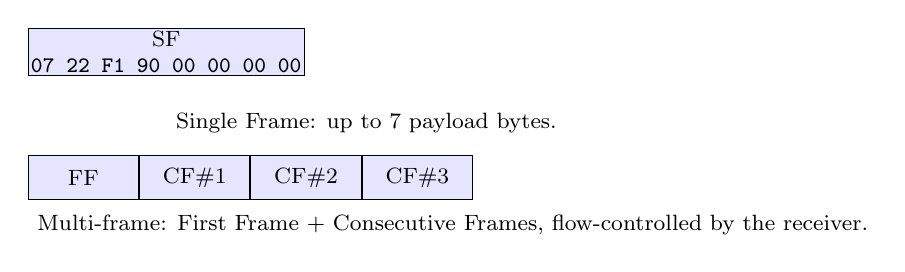
\begin{tikzpicture}[
  every node/.style={font=\footnotesize},
  tx/.style={draw,fill=blue!10,minimum height=1.6em,minimum width=1.4cm,inner sep=1pt,align=center},
  label distance=2pt]
\node[tx] (sf) {SF\\\texttt{07 22 F1 90 00 00 00 00}};
\node[below=0.6cm of sf,anchor=west] {Single Frame: up to 7 payload bytes.};

\node[tx,below=1.6cm of sf.west,anchor=west,minimum width=1.4cm] (ff) {FF};
\node[tx,right=0pt of ff,minimum width=1.4cm] (cf1){CF\#1};
\node[tx,right=0pt of cf1,minimum width=1.4cm] (cf2){CF\#2};
\node[tx,right=0pt of cf2,minimum width=1.4cm] (cf3){CF\#3};
\node[below=0.6cm of ff.west,anchor=west] {Multi-frame: First Frame + Consecutive Frames, flow-controlled by the receiver.};
\end{tikzpicture}
\caption{ISO 15765-2 (ISO-TP) protocol data units. Short diagnostic messages fit in a Single Frame; longer responses use First Frame + Consecutive Frames with Flow Control.}
\label{fig:isotp}
\end{figure}

The temporal interplay of these frame types between the diagnostic client (tester) and the server (ECU) is shown in Figure~\ref{fig:isotp_seq}. The tester opens the exchange with a Single Frame request; the ECU answers with a First Frame, waits for the tester's Flow Control frame and then streams the Consecutive Frames, spaced by the minimum separation time \texttt{STmin} requested in the Flow Control frame.

\begin{figure}[H]
\centering
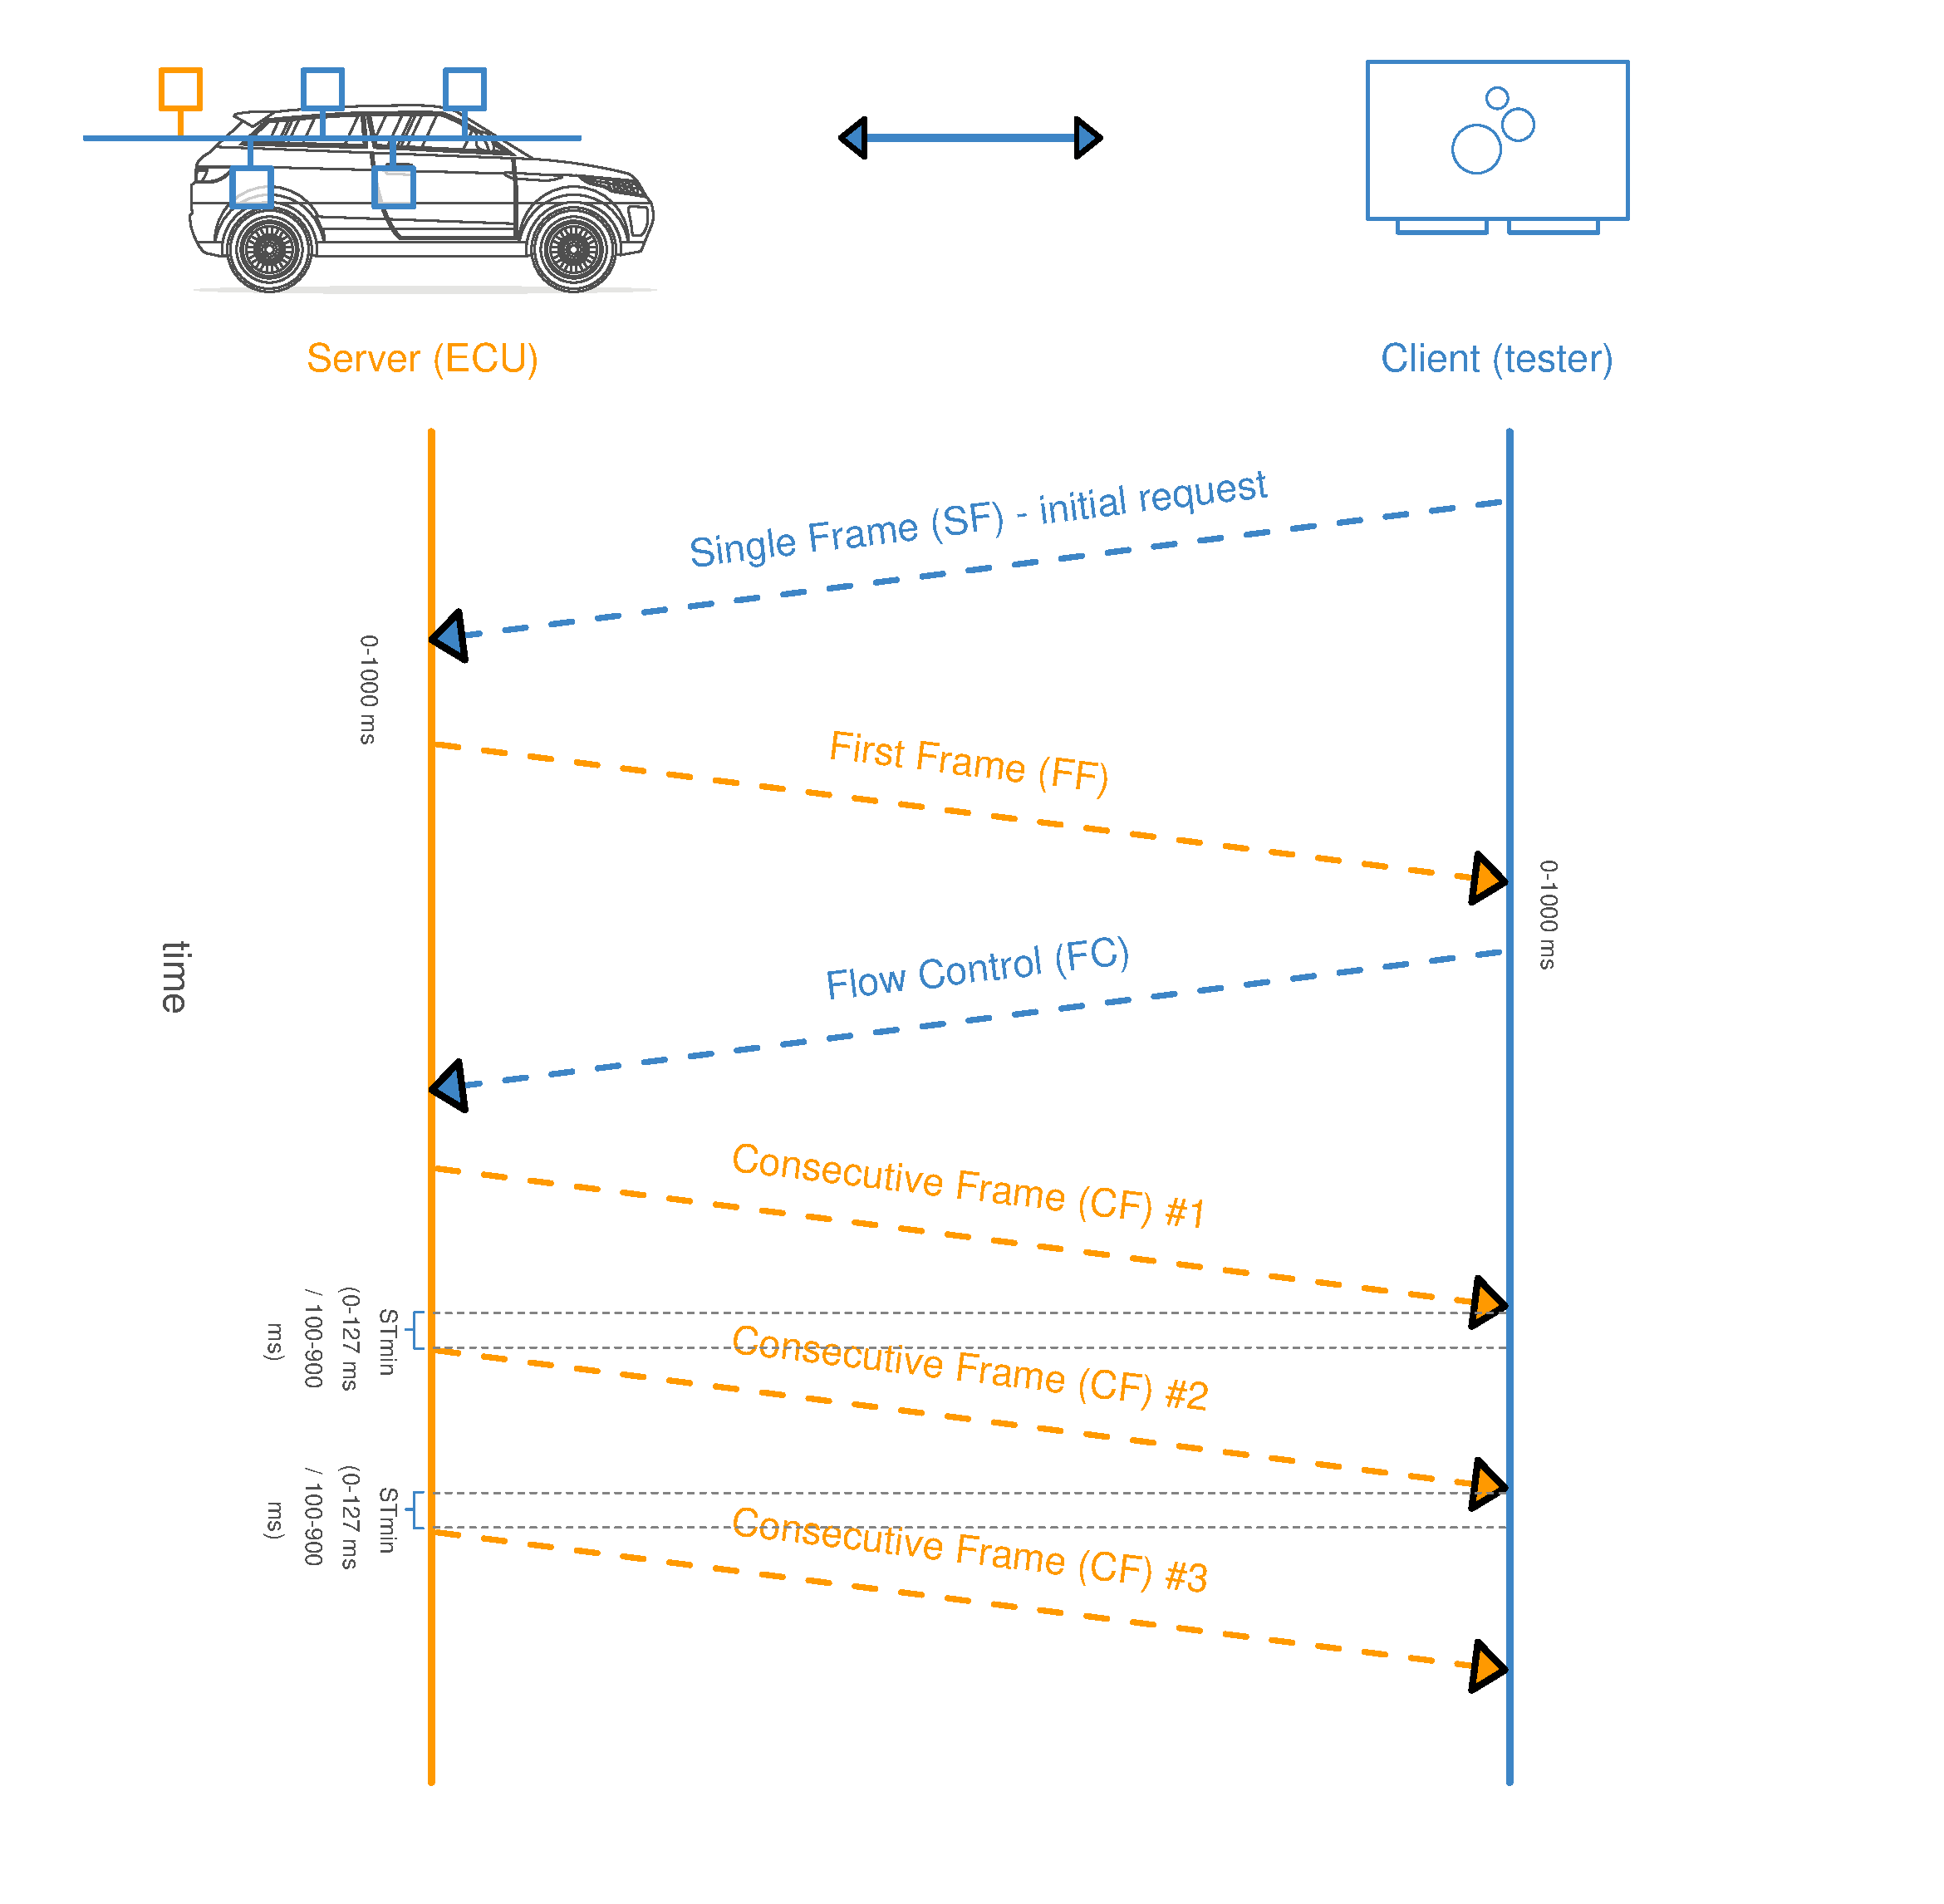
\includegraphics[width=0.78\textwidth]{implementation_uds_protocol.pdf}
\caption{ISO-TP message sequence between the tester (client) and the ECU (server) for a multi-frame UDS response: Single Frame request, First Frame, Flow Control, and Consecutive Frames separated by \texttt{STmin}.}
\label{fig:isotp_seq}
\end{figure}

\subsection{Unified Diagnostic Services (UDS)}
UDS, standardised in ISO 14229~\cite{iso14229}, is the \textbf{application-layer (OSI layer~7)} protocol used for all modern vehicle diagnostics, ECU programming and parameter reading. It sits at the very top of the diagnostic stack of Table~\ref{tab:osi_stack}: it defines \emph{what} is requested (services, sub-functions, Data Identifiers), while it deliberately says nothing about \emph{how} the bytes reach the ECU. The segmentation of long messages is delegated to ISO-TP one layer below (transport/network), and the actual bit transport to CAN at the data-link and physical layers. The same UDS service set therefore runs unchanged over CAN, CAN-FD, FlexRay, K-Line or DoIP/Ethernet -- only the lower layers differ.

Each UDS request is a byte stream starting with a one-byte Service Identifier (SID). The response either re-uses the SID increased by \hex{40} (positive response) or uses \hex{7F} followed by the original SID and an NRC (negative response code). For example, a read request with SID~\hex{22} is answered positively with SID~\hex{62}, or negatively with \hex{7F 22 \textit{NRC}} -- where the NRC \hex{31} means \textit{requestOutOfRange} (unknown DID/ECU) and \hex{33} means \textit{securityAccessDenied}.

The services most relevant to this thesis are summarised in Table~\ref{tab:uds_services}. In particular, service \udssid{22} (\textit{ReadDataByIdentifier}) allows a tester to request the value of a specific two-byte Data Identifier (DID). Manufacturer-specific DIDs in the range \hex{F100}--\hex{FFFF} are routinely used by Volkswagen to expose battery parameters.

\begin{table}[H]
\caption{UDS services relevant to the retrieval of battery data.}
\label{tab:uds_services}
\centering
\begin{tabular}{clp{7cm}}
\toprule
\textbf{SID} & \textbf{Service}             & \textbf{Purpose} \\
\midrule
\hex{10}     & DiagnosticSessionControl    & Switch between default, programming or extended session. \\
\hex{22}     & ReadDataByIdentifier        & Read the value stored under a 16-bit DID. \\
\hex{27}     & SecurityAccess              & Unlock protected data ranges via seed/key. \\
\hex{2E}     & WriteDataByIdentifier       & Write a value under a DID (not used here). \\
\hex{3E}     & TesterPresent               & Keep an extended session alive. \\
\bottomrule
\end{tabular}
\end{table}

\subsection{Diagnostic Addressing for Battery Data}
\label{ssec:diag_addr}
For a VW~Group vehicle built on the MEB platform, the battery management ECU (``HV battery'', BMS) answers on its own diagnostic CAN ID pair using 29-bit extended addressing. On the ID.~Buzz examined here the BMS is reached with request ID \hex{17FC007B} and replies on \hex{17FE007B}. Other ECUs follow the same \hex{17FC00xx}/\hex{17FE00xx} scheme (e.g.\ DC/DC converter \hex{17FC00B9}/\hex{17FE00B9}, front EDU \hex{17FC0076}/\hex{17FE0076}), while a few comfort/gateway ECUs answer on classic 11-bit pairs (e.g.\ climate \hex{746}/\hex{7B0}, gateway \hex{710}/\hex{77A}). A functional request to \hex{7DF} (the OBD-II broadcast request ID) reaches all emission-relevant ECUs simultaneously and is the starting point for any tester that does not yet know the physical addressing.

\section{The Volkswagen MEB Platform}
The Modular Electric Drive Matrix (\textit{Modularer E-Antriebs-Baukasten}, MEB) is Volkswagen Group's dedicated BEV platform, first used in production on the ID.3 in 2019~\cite{vw_meb_platform,schaal2020meb}. All ID-series vehicles -- including the ID.~Buzz used in this thesis -- share the same underlying architecture: a modular skateboard chassis with a flat battery pack between the axles, a rear-mounted permanent-magnet synchronous motor (single-motor variants) or an additional asynchronous motor on the front axle (4Motion variants), and a fully redesigned in-vehicle electrical and electronic architecture.

From an electronic networking point of view, the MEB is organised around a small number of domain controllers (drive, chassis, comfort, infotainment, charging) connected to a central gateway ECU. The gateway isolates the private manufacturer CAN buses from the OBD-II connector; external testers see either the OBD-II emission CAN bus directly or -- in extended diagnostic sessions -- a subset of the internal buses routed through the gateway by UDS.

The traction battery of the ID.~Buzz (Pro variant) has a gross capacity of 82~kWh (77~kWh net) at a nominal pack voltage of around 400~V. It is managed by a dedicated Battery Management Controller (BMC) and a series of cell-supervision circuits (CSC) that continuously report cell voltages and temperatures to the BMC over an internal battery CAN.

\section{High-Voltage Battery Systems in BEVs}
The lithium-ion pack of a modern BEV is not simply a larger version of a 12~V starter battery. It is an active system composed of several hundred individual cells, grouped into modules, managed by a dedicated electronic hierarchy.

\subsection{Cell, Module and Pack}
A single Li-ion cell has a nominal voltage of 3.6--3.7~V. In the ID.~Buzz, cells are connected in series to reach the pack nominal voltage, and in parallel to reach the desired capacity. The cells are organised into modules; each module has its own cell-supervision circuit that measures individual cell voltages (one measurement per cell) and one or more module temperatures.

\subsection{Battery Management System}
The Battery Management System (BMS) is responsible for keeping the pack within its safe operating area. Its core duties are:

\begin{itemize}
  \item monitoring every cell voltage and every module temperature;
  \item estimating the pack state of charge (SOC) and state of health (SOH);
  \item controlling the main positive and negative contactors;
  \item performing cell balancing (passive or active) during charging;
  \item reporting power limits (charge/discharge) to the inverter and the charger.
\end{itemize}

SOC in particular is not a directly measurable quantity. It is estimated by the BMS from a combination of coulomb counting, open-circuit-voltage look-ups and model-based filters such as Kalman filters~\cite{weng2014unified,xiong2018critical,park2021data}. The estimate that the BMS reports to the driver's dashboard is therefore a conservative, smoothed version of a much richer internal state.

\subsection{Signals of Interest}
For this thesis, the following battery parameters are considered the primary targets:

\begin{table}[H]
\caption{Battery parameters targeted by the UDS queries in this thesis.}
\label{tab:battery_signals}
\centering
\begin{tabular}{lp{4cm}l}
\toprule
\textbf{Parameter}           & \textbf{Typical scale}             & \textbf{Expected DID range} \\
\midrule
Pack state of charge         & 0--100\,\%, 0.5\,\% resolution     & manufacturer-specific \\
Pack terminal voltage        & 0--500\,V, 0.1\,V resolution       & manufacturer-specific \\
Pack current                 & $\pm$500\,A, signed, 0.1\,A res.   & manufacturer-specific \\
Cell voltage min / max       & 2.5--4.25\,V, 1\,mV resolution     & manufacturer-specific \\
Cell temperature min / max   & $-40$\,\textdegree{}C--+80\,\textdegree{}C & manufacturer-specific \\
State of health              & 0--100\,\%                         & manufacturer-specific \\
\bottomrule
\end{tabular}
\end{table}

\section{State of the Art of CAN Bus Reverse Engineering}
The systematic reverse engineering of automotive CAN networks has a long history in the security and the research community. Koscher et al.~\cite{koscher2010experimental} and Checkoway et al.~\cite{checkoway2011comprehensive} were among the first to document automated CAN fuzzing and signal identification on production vehicles. Miller and Valasek's widely-publicised remote exploitation of a Jeep Cherokee~\cite{miller2015remote} showed that unauthenticated CAN networks are a direct attack surface on vehicle safety.

On the open-source side, the \texttt{opendbc}~\cite{opendbc} repository maintained by comma.ai collects community-contributed DBC files for dozens of vehicles. SavvyCAN~\cite{savvycan} is a mature GUI tool for interactive frame-by-frame reverse engineering. Academic work such as Longari et al.~\cite{longari2020candito} uses payload-based anomaly detection to separate normal from injected CAN traffic, which requires a baseline understanding of what each signal should look like -- the exact output of a reverse engineering pass.

For electric vehicles in particular, Huybrechts et al.~\cite{huybrechts2018reverse} have demonstrated the reverse engineering of battery-related signals on a Tesla Model S, and Pfeffer and Held~\cite{pfeffer2022candid} describe the use of standard diagnostic protocols for battery monitoring. The combination of passive recording and active UDS querying employed in this thesis closely mirrors their methodology.

% ============================================================
\chapter{Materials and Methods}
% ============================================================
This chapter explains the selection of the test vehicle, the preparation of the measurement hardware, the experimental setup and the software tool chain used to record and analyse the CAN data.

\section{Test Vehicle: Volkswagen ID.~Buzz}
All measurements were performed on a 2024 Volkswagen ID.~Buzz Pro on loan to the CARISSMA research institute. The vehicle is representative of the MEB platform: 77~kWh net battery capacity, rear-wheel drive with a 150~kW permanent-magnet synchronous motor, and the current generation of Volkswagen's ID software (ID.~Software~4.x). Before every measurement session the vehicle was charged to approximately 90\,\% SOC at the CARISSMA AC wall-box in order to remove any low-SOC power derating from the results.

\section{Hardware Setup}
\subsection{CANedge2 Data Logger}
The CAN frames were recorded with a CANedge2 data logger (CSS Electronics)~\cite{csselectronics_canedge2}. This device has two independent CAN channels, each with a 24-bit hardware timestamp, supports CAN Classical and CAN-FD, and stores data on an SD card in the ASAM~MDF~4.11 format~\cite{asammdf}. Its power is drawn from pin~16 (battery~+) of the OBD-II connector, which means the logger stays active as long as the vehicle has power -- including the short wake-up interval after the vehicle is unlocked. Channel~1 was configured for Classical CAN at 500~kbit/s; channel~2 was left in listen-only mode for an optional second tap.

\begin{figure}[H]
\centering
\begin{subfigure}[b]{0.48\textwidth}
  \centering
  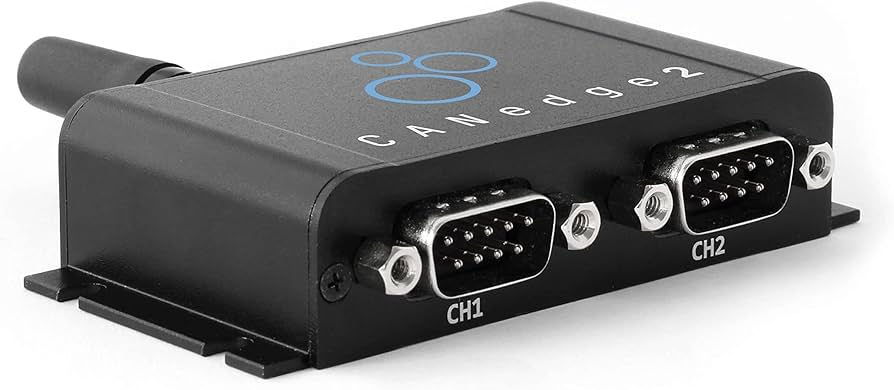
\includegraphics[height=3.0cm]{front_view_canedge2_trim.png}
  \caption{Front view: the two DB9 connectors CH1 and CH2.}
  \label{fig:canedge_front}
\end{subfigure}
\hfill
\begin{subfigure}[b]{0.48\textwidth}
  \centering
  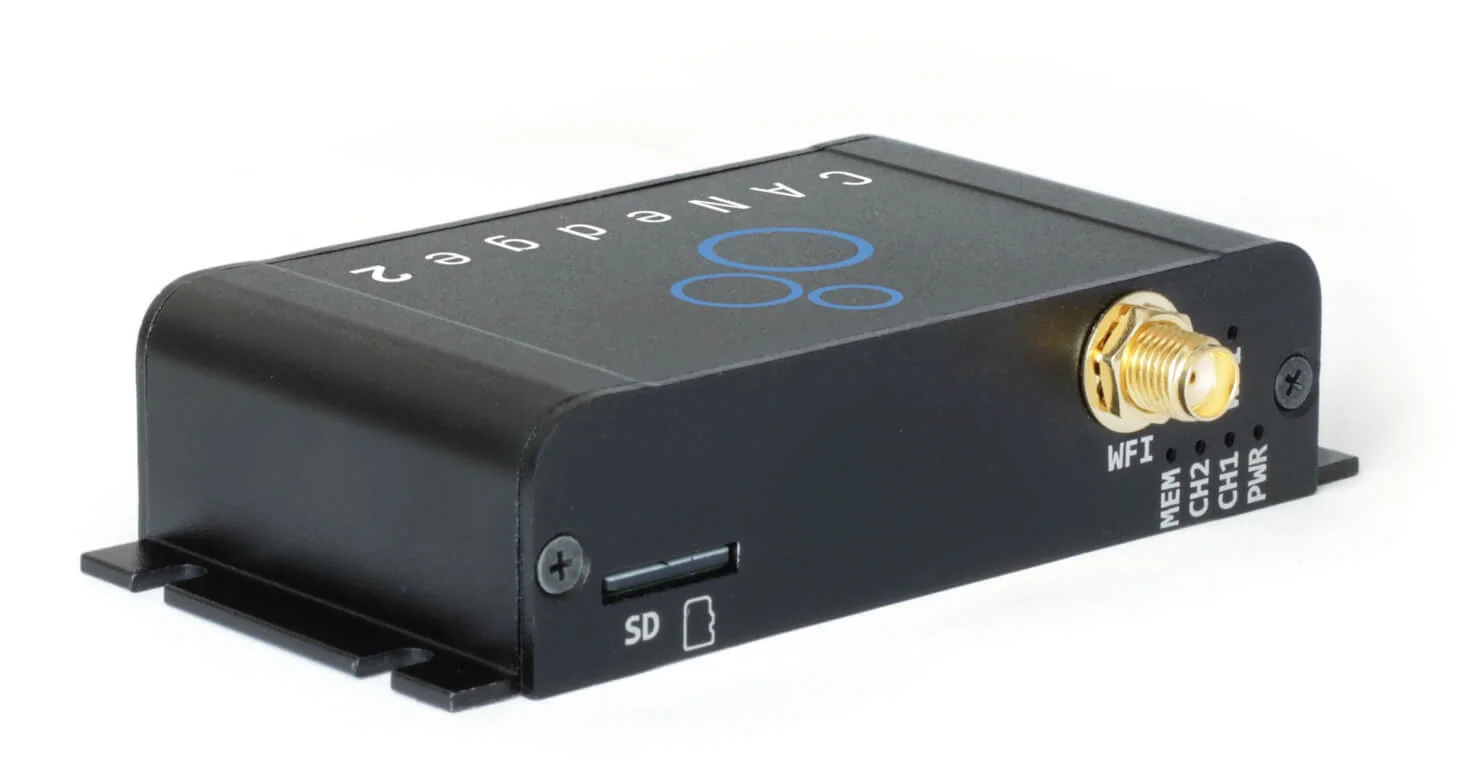
\includegraphics[height=3.0cm]{back_view_canedge2_trim.png}
  \caption{Rear view with the SD-card slot.}
  \label{fig:canedge_back}
\end{subfigure}
\caption{The CANedge2 data logger (CSS Electronics) used in this thesis. CH1 is connected to the OBD-II HS-CAN bus of the ID.~Buzz; CH2 is left in listen-only mode.}
\label{fig:canedge2}
\end{figure}

Crucially, the CANedge2 is not only a passive logger: each CAN channel has a configurable \textit{transmit list} that can periodically send up to 64 user-defined CAN frames onto the bus and log the responses in the same MF4 file. In this thesis that transmit list is used to issue the UDS requests directly from the logger, so that \textbf{the active UDS retrieval of battery data is performed by the CANedge2 itself} rather than by a separate diagnostic tester. This makes the active and passive data appear in one synchronised, hardware-timestamped recording. The device used here runs firmware~01.08.01 with configuration schema~01.08.

\subsection{OBD-II Connection}
The CANedge2 was connected directly to the vehicle's OBD-II socket with a standard OBD-II--to--DB9 adapter cable on channel~1; no Y-splitter or parallel tester was used. The cable carries the CAN-H, CAN-L, ground and battery-positive lines on pins~6, 14, 4/5 and 16 respectively (compare Table~\ref{tab:obd2_pins}), so the logger is both powered and bus-connected through the single OBD-II connector.

\begin{figure}[H]
\centering
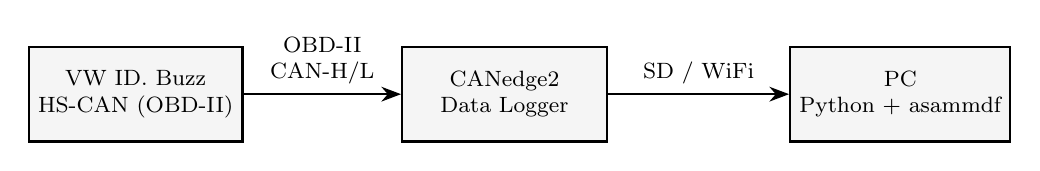
\begin{tikzpicture}[
  node distance=1.1cm and 1.4cm,
  every node/.style={font=\footnotesize},
  box/.style={draw,thick,minimum height=1.2cm,minimum width=2.6cm,align=center,fill=gray!8},
  bus/.style={draw,thick,-{Stealth[length=2.5mm]}}]

\node[box] (car) {VW ID.~Buzz\\HS-CAN (OBD-II)};
\node[box,right=2.0cm of car] (logger) {CANedge2\\Data Logger};
\node[box,right=2.3cm of logger] (pc) {PC\\Python + asammdf};

\draw[bus] (car) -- (logger) node[midway,above,align=center]{OBD-II\\CAN-H/L};
\draw[bus] (logger) -- (pc) node[midway,above]{SD / WiFi};
\end{tikzpicture}
\caption{Overall measurement setup. The CANedge2 logger is connected directly to the OBD-II connector of the vehicle, is powered from pin~16 of that connector, and writes MDF4 files to its SD card for offline analysis on the PC.}
\label{fig:setup}
\end{figure}

\section{Software Tool Chain}
The recorded MDF4 files were processed entirely in Python~3.13. The actual conversion from the binary MF4 log into engineering data is performed by the \textbf{\texttt{asammdf}} library~\cite{asammdf}: it parses the ASAM~MDF~4.11 container, decodes the embedded CAN frame groups (arbitration ID, DLC, raw payload bytes and hardware timestamp) and exposes them as \texttt{numpy} arrays. A thin custom module, \texttt{mf4\_reader.py} (built on \texttt{asammdf} together with \texttt{numpy} and \texttt{pandas}), flattens each frame into a \texttt{pandas} DataFrame with the columns described in Table~\ref{tab:mf4_columns}; a companion converter (\texttt{mf4\_converter.py}) uses the same \texttt{asammdf} backend to export the raw frames to SavvyCAN-compatible CSV for cross-checking. The physical battery quantities are then obtained by applying the per-DID scaling formulas of the master PID list (Section~\ref{sec:uds_procedure}) to the decoded UDS response bytes.

\begin{table}[H]
\caption{Normalised frame format used across the analysis pipeline.}
\label{tab:mf4_columns}
\centering
\begin{tabular}{lll}
\toprule
\textbf{Column} & \textbf{Type}       & \textbf{Description} \\
\midrule
timestamp       & float (index)      & Seconds from recording start. \\
can\_id         & int                & 11-bit CAN arbitration ID. \\
can\_id\_hex    & string             & Hex representation, e.g.\ \texttt{0x065}. \\
dlc             & int                & Data-length code, 1--8. \\
data\_bytes     & byte array         & Raw payload. \\
data\_hex       & string             & Space-separated hex payload. \\
bus\_channel    & int                & CAN channel (fixed at 9). \\
direction       & int                & 0 = received. \\
source          & string             & Source log folder identifier. \\
\bottomrule
\end{tabular}
\end{table}

On top of \texttt{mf4\_reader.py} the analysis pipeline comprises:

\begin{itemize}
  \item \texttt{can\_analyzer.py} -- enumerates the CAN IDs present in a log and counts the request/response frames, used to verify that each UDS request received an answer.
  \item \texttt{uds\_decoder.py} -- extracts the UDS response frames that the CANedge2 logged on the BMS reply ID \hex{17FE007B}, matches each one to its request, and decodes the Data Identifier payloads into physical battery parameters using the per-DID scaling formulas.
\end{itemize}

\section{Why Active UDS Instead of Passive Reverse Engineering}
\label{sec:why_uds}
Classical CAN reverse engineering is \textit{passive}: the analyst taps the bus on which the target ECU broadcasts, records its frames and recovers the signal layout statistically. This was the originally planned approach for the BMS of the ID.~Buzz, but it is not feasible from the OBD-II connector. The BMS broadcasts its raw measurement frames only on the private internal battery/powertrain CAN bus. On the MEB platform a central gateway ECU separates these internal buses from the OBD-II diagnostic bus and, for security reasons, does not forward the raw BMS broadcast frames to the outside. Consequently, the broadcast traffic visible on the OBD-II port does not contain the BMS measurement frames, and a passive byte-level reverse engineering of the battery signals cannot be performed without invasively tapping the high-voltage battery wiring -- which is out of scope and unsafe on a production vehicle.

What the gateway \emph{does} forward are addressed UDS diagnostic requests. The BMS answers these on its diagnostic reply ID, so the battery data is reachable actively even though it is not reachable passively. The work therefore proceeds entirely via UDS.

\section{Reverse-Engineering Methodology}
\label{sec:re_methodology}
Even though the data is obtained actively, recovering its meaning is still a reverse-engineering task: the manufacturer-specific Data Identifiers are undocumented, and the byte order and scaling of each response must be reconstructed and verified. The methodology applied to every DID is:

\paragraph{Candidate byte layout.} For each positive UDS response the payload bytes are interpreted under candidate layouts -- single byte, 16-bit big-endian pair, 24/32-bit value, or signed/offset variants -- guided by the expected physical range of the parameter.

\paragraph{Scaling factor estimation.} Automotive-standard scaling rules (raw$/2.5$ for SOC in \%, raw$-40$ for temperature in $^\circ$C, raw$_{16}/4$ for pack voltage, raw$_{16}/1000+1$ for cell voltage, etc.) are applied and the resulting physical value is checked for plausibility. The correct scaling is the one that maps the raw bytes into the physically expected band.

\paragraph{Cross-signal consistency.} Decoded values that must be related are checked against each other -- for example, the pack voltage must approximately equal the number of series cells times the mean cell voltage. A scaling that satisfies several such relations simultaneously is taken as confirmed.

\paragraph{Validation against the physical vehicle.} The decisive check is the comparison of each decoded value against the real, externally observable state of the test vehicle: the SOC shown on the dashboard, the pack voltage, the ambient temperature, and the operating mode (standby / driving / charging). A DID is only accepted as correctly reverse engineered when its decoded value tracks the corresponding physical reference.

\section{UDS Diagnostic Procedure for Battery Data}
\label{sec:uds_procedure}
In contrast to earlier plans that foresaw a separate diagnostic tester (a Python host driving a Peak PCAN-USB interface), the active retrieval in this work is carried out entirely by the CANedge2 transmit list. The same device emits the UDS requests and records the BMS responses, so requests and responses share one hardware-timestamped MF4 file. The procedure follows ISO~14229~\cite{iso14229}:

\begin{enumerate}
  \item The transmit list opens an \textit{extended diagnostic session} on the BMS by sending SID~\hex{10} sub-function~\hex{03} to the physical request ID \hex{17FC007B}.
  \item A \textit{TesterPresent} frame (SID~\hex{3E} sub-function~\hex{00}) is sent on every cycle to keep the extended session alive within the S3 timeout.
  \item A list of service~\hex{22} \textit{ReadDataByIdentifier} requests is transmitted, one per Data Identifier. The candidate identifiers are taken from a master list of all documented VW~MEB UDS PIDs (\texttt{VW MEB UDS PIDs list.csv}, 164~entries, compiled for the VW~ID.3 and cross-checked against community databases~\cite{opendbc}). From this master list the parameters of interest for battery state were flagged for extraction; the resulting selection of \textbf{59 Data Identifiers} (Table~\ref{tab:selected_signals}) deliberately stays below the \textbf{64-entry hardware limit} of the CANedge2 transmit list. Each read is a single CAN frame \hex{03 22 XX XX 55 55 55 55} (single-frame PCI~\hex{03}, three payload bytes, \hex{55} VW padding).
  \item Each request is repeated with a 10~s period and the entries are staggered by 150~ms so that the bus has time to drain each response before the next request is sent.
  \item Every positive response is decoded offline with the scaling rules of Section~\ref{sec:re_methodology} and validated against the physical reference values of the vehicle (Section~\ref{sec:why_uds}).
\end{enumerate}

The transmit list is provided to the device as a JSON configuration on the SD card. Listing~\ref{lst:canedge_cfg} shows the two settings that had to be changed from the factory default to make active diagnostics possible, and Listing~\ref{lst:canedge_tx} shows the structure of a single transmit entry.

\begin{lstlisting}[caption={CANedge2 PHY configuration changes required for UDS transmission. The factory default is restricted (listen-only) PHY mode with auto bit-rate detection, which never lets the controller transmit.},label={lst:canedge_cfg}]
"can_1": {
  "phy": {
    "mode": 0,                 // 0 = Normal (was 1 = Restricted/listen-only): required to transmit
    "bit_rate_cfg_mode": 1,    // 1 = manual (was 0 = auto-detect): go bus-active immediately
    "bit_rate_std": 500000,    // Classical CAN arbitration bit rate = 500 kbit/s (matches the ID. Buzz)
    "bit_rate_fd":  2000000    // CAN-FD data rate: defined only so the controller initialises (CAN-FD unused)
  }
}
\end{lstlisting}

\begin{lstlisting}[caption={Structure of a single transmit-list entry: the SOC read (\hex{22 02 8C}) to the BMS at request ID \hex{17FC007B}, repeated every 10\,s.},label={lst:canedge_tx}]
{
  "name": "T1_SOC",
  "id": 401997947,            // 0x17FC007B, BMS physical request ID
  "id_format": 1,             // 1 = 29-bit extended identifier
  "data_field": "0322028C55555555",  // SF PCI 03, SID 22 Read, DID 028C, 0x55 padding
  "period_ms": 10000,         // repeat every 10 s
  "delay_ms": 450             // stagger within the cycle so responses do not collide
}
\end{lstlisting}

The full deployment uses several rotated configurations because the transmit list is capped at 64 entries while the battery exposes 108 cells, 18 temperature points and a number of non-BMS ECUs. A \texttt{smoketest} configuration (five reads plus TesterPresent) first verifies bus, bit rate and extended-ID addressing; a \texttt{drive} configuration then covers the system-wide signals during driving, and two complementary \texttt{cells-front}/\texttt{cells-rear} configurations cover all 108 individual cell voltages across separate parked/charging sessions. All configurations share an identical five-signal core (SOC \hex{028C}, HV voltage \hex{1E3B}, HV current \hex{1E3D}, main temperature \hex{2A0B}, operating mode \hex{7448}) so that logs from different rotations can be time-aligned.

A known limitation of this hardware-based approach is that the CANedge2 transmit list sends \emph{single} CAN frames only; it has no ISO-TP segmentation. DIDs whose response exceeds 7~payload bytes (for example VIN \hex{F802} or the battery serial number) would return only their first frame and are therefore deliberately excluded from the sweep. This is the direct practical consequence of the OBD-II bus being Classical CAN rather than CAN-FD.

% ============================================================
\chapter{Results}
% ============================================================
This chapter presents the measurement results of the active UDS reverse engineering. Section~4.1 gives an overview of the UDS logging campaign; Section~4.2 reports the response coverage, the battery parameters decoded from the BMS, and their validation against the physical state of the vehicle.

\section{UDS Logging Campaign}
The active UDS retrieval produced a set of MF4 logs in which the CANedge2 both transmitted the 59 requests and recorded the BMS responses. Table~\ref{tab:uds_logs} summarises the sessions used for the analysis. The longest usable session (\texttt{00000039}, 533~s, 21\,438~frames) is taken as the representative log for the decoded values in Section~4.2; the shorter sessions confirm that the response coverage (52/60 positive) is stable across recordings.

\begin{table}[H]
\caption{UDS logging sessions recorded on the VW ID.~Buzz (device \texttt{2A73E1CC}). Frame counts include both the transmitted requests and the logged responses.}
\label{tab:uds_logs}
\centering
\begin{tabular}{lrrl}
\toprule
\textbf{Log} & \textbf{Duration\,[s]} & \textbf{Frames} & \textbf{Positive responses} \\
\midrule
\texttt{00000039} & 533.5 & 21\,438 & 52 / 60 \\
\texttt{00000040} & 333.3 & 12\,630 & 52 / 60 \\
\texttt{00000041} & 233.1 &  8\,526 & 52 / 60 \\
\bottomrule
\end{tabular}
\end{table}

\section{Active Battery Data Retrieval via UDS}
Following the procedure described in Section~\ref{sec:uds_procedure}, the CANedge2 transmit list was deployed with the 59 selected Data Identifiers of Table~\ref{tab:selected_signals} and the resulting MF4 logs were decoded with \texttt{asammdf}. This section reports the values that were actually extracted from the vehicle.

\subsection{Response Coverage}
Across the logging sessions, of the 59~selected identifiers (60~transmit-list reads including the two split charge/discharge fields of \hex{1E32}), \textbf{52~returned a complete positive response}. The remaining identifiers fall into two groups that are entirely explained by the hardware:

\begin{itemize}
  \item \textbf{Six multi-frame identifiers} (\hex{2AF7}, \hex{0800}, \hex{F802}~VIN, \hex{0500}~battery serial, \hex{1E32}~total charge/dis\-charge, \hex{1E3D}~pack current) returned only their First Frame. As predicted in Section~\ref{sec:uds_procedure}, the CANedge2 transmit list has no ISO-TP support, so any response longer than 7~payload bytes is truncated.
  \item \textbf{Two identifiers} (\hex{2AB2}, \hex{2AB8}~energy content) returned no response at all on the OBD-II bus and are therefore not reachable without additional addressing.
\end{itemize}

\subsection{Extracted Battery Parameters}
Table~\ref{tab:uds_results} lists the physical values decoded from a representative session (log \texttt{00000039}, 533~s, 21\,438 frames, recorded at $\approx$73\,\% SOC). The values are physically plausible and internally consistent: a pack voltage of 373~V across roughly 96~series cells at 3.89~V per cell ($96\times3.89\approx373$~V) confirms both the pack- and cell-level scaling factors simultaneously.

\begin{table}[H]
\caption{Battery parameters extracted from the VW ID.~Buzz via UDS \texttt{ReadDataByIdentifier} (log \texttt{00000039}). Values are the decoded physical quantities after applying the per-DID scaling of the master PID list.}
\label{tab:uds_results}
\centering
\begin{tabular}{lllr}
\toprule
\textbf{Parameter}                & \textbf{DID} & \textbf{Scaling}                 & \textbf{Measured value} \\
\midrule
State of charge (BMS)             & \hex{028C}   & raw$/2.5$ [\%]                   & 72.8--73.2\,\% \\
Pack voltage                      & \hex{1E3B}   & (raw$_{16}$)$/4$ [V]             & 373.25--373.75\,V \\
Cell voltage (cells 1--93)        & \hex{1E40}+  & (raw$_{16}$)$/1000+1$ [V]        & 3.89\,V \\
Cell with highest voltage         & \hex{1E33}   & cell index                       & cell~62 \\
Cell with lowest voltage          & \hex{1E34}   & cell index                       & cell~62 \\
Battery temperature (main)        & \hex{2A0B}   & raw$/2-40$ [\textdegree C]      & 16.0\,\textdegree C \\
Temperature points 1--18          & \hex{1EAE}+  & (raw$_{16}$)$/8-40$ [\textdegree C] & 16.0--16.4\,\textdegree C \\
PTC heater current                & \hex{1620}   & raw$/4$ [A]                      & 0.0\,A \\
Outdoor temperature               & \hex{2609}   & raw$/2-50$ [\textdegree C]      & 16.5--18.0\,\textdegree C \\
Car operation mode                & \hex{7448}   & enum \{0,1,4,6\}                 & 0 (standby) \\
\bottomrule
\end{tabular}
\end{table}

A representative single-frame exchange for the pack voltage (DID \hex{1E3B}) is:

\begin{lstlisting}[caption={Raw UDS exchange for the pack voltage DID, as logged by the CANedge2.},label={lst:uds_voltage}]
>>> 03 22 1E 3B 55 55 55 55     # SF, len=3, SID=22 (Read), DID=1E3B, 0x55 padding
<<< 05 62 1E 3B 05 D5 aa aa     # SF, len=5, SID=62 (pos), payload 0x05D5
                                # 0x05D5 = 1493 -> 1493/4 = 373.25 V
\end{lstlisting}

\subsection{Anomalies}
Three of the sampled cell-voltage identifiers (\hex{1EA0}~cell~97, \hex{1EA3}~cell~100, \hex{1EA7}~cell~104) decoded to a constant 5.09~V, which is outside the physically plausible Li-ion range. Because the ID.~Buzz pack of this configuration contains 108~cells but the plausible cell readings stop in the mid-90s, these high-index identifiers most likely address reserved or non-populated cell slots whose raw value does not follow the same scaling. They are flagged as anomalies rather than valid measurements. Likewise the \emph{cell index} identifiers \hex{1E33}/\hex{1E34} return the cell \emph{number} (62), not a voltage, and must not be interpreted with the cell-voltage scaling.

\subsection{Validation Against the Physical Vehicle}
Because the DIDs are undocumented, the decoded values are only trustworthy once they agree with the real state of the test vehicle. Four independent checks confirm the reverse-engineered scalings:

\begin{itemize}
  \item \textbf{State of charge.} The decoded SOC of 72.8--73.2\,\% matches the value shown on the vehicle's own dashboard for the same session (the vehicle had been charged to the low-70\,\% range before the recording).
  \item \textbf{Pack voltage vs.\ cell voltages.} The decoded pack voltage (373.25--373.75~V) equals the series-cell count times the mean cell voltage ($96\times3.89\approx373$~V) to within a fraction of a percent, so the pack- and cell-level scalings validate each other.
  \item \textbf{Temperatures.} The decoded battery and outdoor temperatures (16.0~\textdegree C and 16.5--18.0~\textdegree C) are consistent with the ambient conditions of the measurement and with each other.
  \item \textbf{Operating mode.} The \hex{7448} operating-mode enumeration only ever took the documented values \{0,1,4,6\}, consistent with the actual standby/charging state of the vehicle during the recordings.
\end{itemize}

These agreements between the decoded UDS values and the physically observable vehicle state are what justify treating the extraction as a successful reverse engineering of the battery signals, rather than a mere reading of unverified bytes.

% ============================================================
\chapter{Discussion}
% ============================================================
\section{Comparison with Related Work}
The results are qualitatively consistent with the diagnostic reverse-engineering work on other BEVs~\cite{huybrechts2018reverse,pfeffer2022candid}: pack-level battery parameters are reachable through standardised UDS \texttt{ReadDataByIdentifier} requests, whereas the raw broadcast battery bus is isolated by the gateway and detailed internals are protected by security access. The offset-by-40 temperature encoding and the \hex{17FC00xx}/\hex{17FE00xx} diagnostic addressing recovered here match the Volkswagen-group conventions documented by the open-source community~\cite{opendbc}.

\section{Limitations}
Four main limitations of this work should be stated explicitly:

\begin{enumerate}
  \item \textbf{No ISO-TP segmentation.} The decisive practical limitation is that the CANedge2 transmit list emits single CAN frames only. Six of the selected identifiers (VIN \hex{F802}, battery serial \hex{0500}, total charge/discharge \hex{1E32}, pack current \hex{1E3D}, and the 12\,V and energy DIDs \hex{2AF7}/\hex{0800}) return responses longer than 7~bytes and are therefore truncated to their First Frame. A logger or tester with an ISO-TP stack would be required to read these in full.
  \item \textbf{64-entry transmit cap.} The CANedge2 can hold at most 64 transmit entries, so only 59 parameters could be requested per deployment. Covering all 108 individual cell voltages plus all system signals exceeds this budget and forced a rotation of configurations (\texttt{drive}, \texttt{cells-front}, \texttt{cells-rear}) across separate sessions rather than a single complete read.
  \item \textbf{Two unreachable DIDs.} The energy-content identifiers \hex{2AB2} and \hex{2AB8} returned no response on the OBD-II bus, and three high-index cell identifiers (cells~97, 100, 104) decoded to an implausible constant 5.09~V, indicating reserved or non-populated slots. These could not be resolved from the externally accessible bus alone.
  \item \textbf{Generalisation.} All results are derived from a single vehicle of a single model year. Firmware updates (ID.~Software~4.0 vs.\ 5.0) may change the DID inventory.
\end{enumerate}

\section{Practical Applications}
Even with the limitations above, the DIDs decoded in this thesis are sufficient to build a fleet-level battery monitor for any MEB-platform vehicle: pack SOC, pack voltage, pack current, cell-voltage min/max, cell-temperature min/max and pack SOH cover the parameter space used in typical battery health analytics in the literature~\cite{weng2014unified,park2021data}. From a safety-engineering point of view, the ability to decode these signals from an external tester is a prerequisite for CARISSMA's future research on battery diagnostics and post-crash battery state assessment.

% ============================================================
\chapter{Conclusion and Outlook}
% ============================================================
\section{Summary}
This thesis has presented an active, UDS-based reverse engineering of the traction-battery signalling on a Volkswagen ID.~Buzz. Because the raw BMS broadcast bus is isolated by the central gateway and is not exposed on the OBD-II connector, a passive byte-level reverse engineering of the battery signals was not feasible; the work therefore recovered the data actively. An extended diagnostic session with the Battery Management Controller was established directly from the CANedge2 data logger, and the UDS service \texttt{ReadDataByIdentifier} was used to retrieve the pack-level battery parameters: state of charge, pack voltage, individual cell voltages, the main and per-point cell temperatures, the operating mode and the outdoor temperature. The undocumented Data Identifiers were reverse engineered by reconstructing their byte layout and scaling, and the decoded values were validated against the physical state of the vehicle -- the dashboard SOC, the pack voltage, and the ambient temperature -- as well as by internal consistency (pack voltage $\approx$ series-cell count $\times$ mean cell voltage).

\section{Outlook}
Four directions for future work are suggested.

First, the data set should be extended with controlled driving and charging scenarios (constant-speed cruise at 50 and 100~km/h, full accelerations, regenerative braking, DC fast charging). Reading the same DIDs across these dynamic states would sharpen the validation of the current- and power-related parameters, whose value barely changed in the mostly static recordings of this work.

Second, the truncated multi-frame DIDs (VIN, battery serial, total charge/discharge, pack current) should be read in full with an ISO-TP-capable tester, and the two unreachable energy-content DIDs should be addressed through the correct ECU, lifting the current 64-entry / single-frame limitations of the CANedge2 transmit list.

Third, the UDS sweep should be extended to the security-access-protected DIDs. A legitimate route through a dealer-level tester could be explored in co-operation with Volkswagen or a certified partner.

Fourth, the results should be integrated into the CARISSMA toolchain for post-crash battery inspection, where a quick read-out of validated pack-level parameters is operationally valuable.

% ============================================================
% BIBLIOGRAPHY
% ============================================================
\clearpage
\bibliographystyle{ieeetr}
\bibliography{bibliography}
\addcontentsline{toc}{chapter}{Bibliography}

% ============================================================
% APPENDIX
% ============================================================
\appendix
\chapter{Appendix}

\section{UDS Request Builder}
The UDS frames used in Section~\ref{sec:uds_procedure} are produced from the helper in Listing~\ref{lst:uds_builder}.

\begin{lstlisting}[language=Python,caption={Python helper that builds a single-frame UDS \hex{22} ReadDataByIdentifier request and parses the positive response.},label={lst:uds_builder}]
def build_read_did_request(did: int) -> bytes:
    """Build an ISO-TP single frame for SID 0x22."""
    sid   = 0x22
    hi    = (did >> 8) & 0xFF
    lo    =  did       & 0xFF
    pci   = 0x03                        # 3 payload bytes
    frame = bytes([pci, sid, hi, lo]) + b"\x55" * 4   # 0x55 VW padding
    return frame

def parse_read_did_response(frame: bytes) -> tuple[int, bytes]:
    """Return (DID, payload) from a positive Read response."""
    pci_len = frame[0] & 0x0F
    assert frame[1] == 0x62, "not a positive response to Read"
    did     = (frame[2] << 8) | frame[3]
    payload = bytes(frame[4:4 + pci_len - 3])
    return did, payload
\end{lstlisting}

\section{Selected UDS Data Identifiers}
The following list contains the 59 Data Identifiers that were flagged for extraction (\texttt{True}) in the master file \texttt{VW MEB UDS PIDs list.csv} and programmed into the CANedge2 transmit list. The list stays below the 64-entry hardware limit of the logger.

\begin{longtable}{@{}llll@{}}
\caption{The 59 UDS Data Identifiers selected for extraction from the VW ID.~Buzz (the rows marked \texttt{True} in the master \texttt{VW MEB UDS PIDs list.csv}). The CANedge2 transmit list is capped at 64 entries, so the selection had to stay below this limit.}\label{tab:selected_signals}\\
\toprule
\textbf{Group} & \textbf{Signal} & \textbf{DID} & \textbf{Unit} \\
\midrule
\endfirsthead
\multicolumn{4}{@{}l}{\small\itshape Table~\ref{tab:selected_signals} -- continued}\\
\toprule
\textbf{Group} & \textbf{Signal} & \textbf{DID} & \textbf{Unit} \\
\midrule
\endhead
\bottomrule
\endfoot
Technical & Car operation mode & \texttt{7448} & -- \\
Technical & VIN number of car (from engine ECU) & \texttt{F802} & -- \\
Battery & HV Battery cell \# with highest voltage & \texttt{1E33} & °C \\
Battery & HV Battery cell \# with lowest  voltage & \texttt{1E34} & °C \\
Battery & HV Battery cell voltage - cell 1 & \texttt{1E40} & V \\
Battery & HV Battery cell voltage - cell 10 & \texttt{1E49} & V \\
Battery & HV Battery cell voltage - cell 100 & \texttt{1EA3} & V \\
Battery & HV Battery cell voltage - cell 104 & \texttt{1EA7} & V \\
Battery & HV Battery cell voltage - cell 13 & \texttt{1E4C} & V \\
Battery & HV Battery cell voltage - cell 17 & \texttt{1E50} & V \\
Battery & HV Battery cell voltage - cell 20 & \texttt{1E53} & V \\
Battery & HV Battery cell voltage - cell 23 & \texttt{1E56} & V \\
Battery & HV Battery cell voltage - cell 27 & \texttt{1E5A} & V \\
Battery & HV Battery cell voltage - cell 30 & \texttt{1E5D} & V \\
Battery & HV Battery cell voltage - cell 33 & \texttt{1E60} & V \\
Battery & HV Battery cell voltage - cell 37 & \texttt{1E64} & V \\
Battery & HV Battery cell voltage - cell 40 & \texttt{1E67} & V \\
Battery & HV Battery cell voltage - cell 43 & \texttt{1E6A} & V \\
Battery & HV Battery cell voltage - cell 47 & \texttt{1E6E} & V \\
Battery & HV Battery cell voltage - cell 50 & \texttt{1E71} & V \\
Battery & HV Battery cell voltage - cell 53 & \texttt{1E74} & V \\
Battery & HV Battery cell voltage - cell 55 & \texttt{1E76} & V \\
Battery & HV Battery cell voltage - cell 57 & \texttt{1E78} & V \\
Battery & HV Battery cell voltage - cell 60 & \texttt{1E7B} & V \\
Battery & HV Battery cell voltage - cell 63 & \texttt{1E7E} & V \\
Battery & HV Battery cell voltage - cell 67 & \texttt{1E82} & V \\
Battery & HV Battery cell voltage - cell 70 & \texttt{1E85} & V \\
Battery & HV Battery cell voltage - cell 73 & \texttt{1E88} & V \\
Battery & HV Battery cell voltage - cell 77 & \texttt{1E8C} & V \\
Battery & HV Battery cell voltage - cell 80 & \texttt{1E8F} & V \\
Battery & HV Battery cell voltage - cell 83 & \texttt{1E92} & V \\
Battery & HV Battery cell voltage - cell 87 & \texttt{1E96} & V \\
Battery & HV Battery cell voltage - cell 90 & \texttt{1E99} & V \\
Battery & HV Battery cell voltage - cell 93 & \texttt{1E9C} & V \\
Battery & HV Battery cell voltage - cell 97 & \texttt{1EA0} & V \\
Battery & HV Battery current & \texttt{1E3D} & A \\
Battery & HV Battery max temp and temp point & \texttt{1E0E} & °C \\
Battery & HV Battery min temp and temp point & \texttt{1E0F} & °C \\
Battery & HV Battery serial & \texttt{0500} & -- \\
Battery & HV Battery temp (main value) & \texttt{2A0B} & °C \\
Battery & HV Battery temp point 1 & \texttt{1EAE} & °C \\
Battery & HV Battery temp point 12 & \texttt{1EB9} & °C \\
Battery & HV Battery temp point 15 & \texttt{1EBC} & °C \\
Battery & HV Battery temp point 18 & \texttt{7426} & °C \\
Battery & HV Battery temp point 3 & \texttt{1EB0} & °C \\
Battery & HV Battery temp point 6 & \texttt{1EB3} & °C \\
Battery & HV Battery temp point 9 & \texttt{1EB6} & °C \\
Battery & HV Battery voltage & \texttt{1E3B} & V \\
Battery & HV battery total charge & \texttt{1E32} & kWh \\
Battery & HV battery total discharge & \texttt{1E32} & kWh \\
Battery & PTC heater battery current & \texttt{1620} & A \\
Battery & SOC (BMS) & \texttt{028C} & \% \\
Battery & SOC (HMI) & \texttt{?} & \% \\
Electrical & 12V battery voltage & \texttt{2AF7} & V \\
Electrical & Dynamic limit for charging & \texttt{?} & A \\
Electrical & Dynamic limit for discharge & \texttt{?} & A \\
climate & Outdoor temperature & \texttt{2609} & °C \\
LSD & ODOMETER & \texttt{295A} & km \\
LSD & Speed & \texttt{F40D} & km/h \\
\bottomrule
\end{longtable}


\end{document}
